\documentclass[tikz]{standalone}
\usepackage[utf8]{inputenc}

\definecolor{DarkBlue}{rgb}{0.0,0.0,0.6}
\definecolor{DarkRed}{rgb}{0.7,0.2,0.2}

\begin{document}

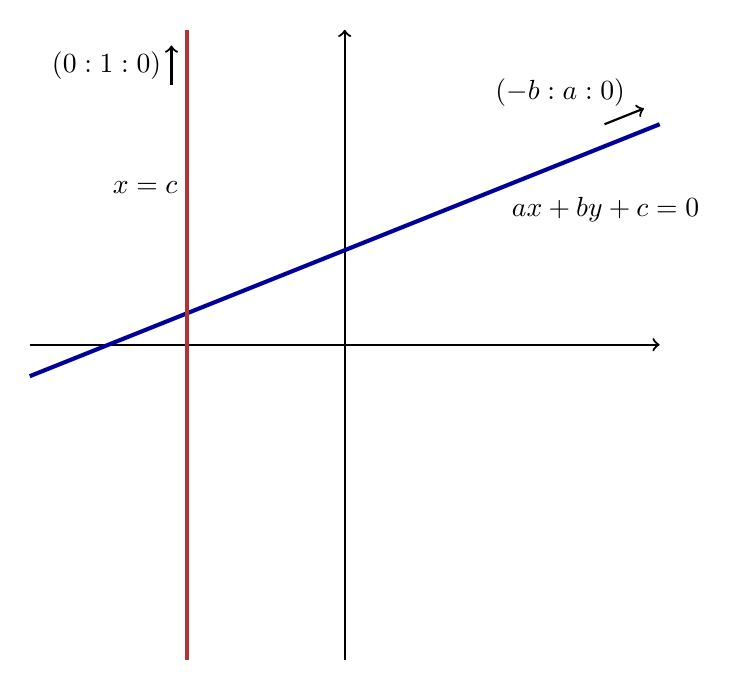
\begin{tikzpicture}
\draw[thick,->] (-4, 0) -- (4,0);
\draw[thick,->] (0,-4) -- (0,4);

\draw[line width=1.5pt,domain={-4:4},DarkBlue] plot (\x, .4*\x + 1.2);
\node[below right] at (2,2) {$ax+by+c=0$};
\draw[<-,shift={(-.2,.2)},thick] (4,2.8) --++ (-.5,-.2) node[midway,above left,xshift=4pt] {$(-b:a:0)$};
\draw[line width=1.5pt,DarkRed] (-2,-4) -- (-2,4);
\node[left] at (-2,2) {$x=c$};
\draw[->,thick] (-2.2,3.3) --++ (0,.5) node[midway,left] {$(0:1:0)$};
\end{tikzpicture}

\end{document}